\section{Experiment}
\label{sec:experiment}

We looked maximum a posteriori learning of the logistic regression classifier in class. In particular, we showed that learning the classifier is equivalent to the following optimization problem: $\min_{\bw} \Bigl\{\sum_{i=1}^m \log(1+ \exp(-y_i\bw^T\bx_i)) + \frac{1}{\sigma^2}\bw^T\bw\Bigr\}$.

In this question, you will derive the stochastic gradient descent algorithm for the logistic
regression classifier, and also implement it with cross-validation. 
%Detailed instructions on cross-validation procedure can be found in homework 1, and instructions on SGD can be found in homework 5.

\begin{enumerate}
\item ~[5 points] What is the derivative of the function $g(\bw) = \log(1+ \exp(-y_i\bw^T\bx_i))$ with respect to the weight vector?

\begin{equation*}
\begin{aligned}
\triangledown g(\bw) &= \triangledown \log(1+ \exp(-y_i\bw^T\bx_i))\\
&= \frac{1}{1+ \exp(-y_i\bw^T\bx_i)} \exp(-y_i\bw^T\bx_i) (-y_i x_i)\\
&= \frac{-y_i \bx_i \exp(-y_i\bw^T\bx_i)}{1+ \exp(-y_i\bw^T\bx_i)} = \frac{-y_i \bx_i}{1+ \exp(y_i\bw^T\bx_i)}
\end{aligned}
\end{equation*}


\item ~[5 points] The inner most step in the SGD algorithm is the gradient update where we use a single example instead of the entire dataset to compute the gradient. Write down the objective where the entire dataset is composed of a single example, say $(\bx_i, y_i)$. Derive the gradient of this objective with respect to the weight vector.

We need to find the weight $\bw$ that minimizes the expression given above in the question. The objective when the entire dataset consists of a single example $(\bx_i, y_i)$ is $J(\bw) = \log(1+ \exp(-y_i\bw^T\bx_i)) + \frac{1}{\sigma^2}\bw^T\bw$\\


The derivative of the first part has already been derived above. The gradient of this objective with respect to the weight vector is $\triangledown J(\bw) = \frac{-y_i \bx_i}{1+ \exp(y_i\bw^T\bx_i)} + \frac{2\bw}{\sigma^2}$

\item ~[10 points] Write down the pseudo code for the stochastic gradient algorithm using the gradient from previous part.

\begin{minipage}{\linewidth}
  \begin{algorithm}[H]
    \caption{Stochastic Gradient Descent }\label{AlgSGD}
    \begin{algorithmic}[1]
      \Procedure{SGD}{$ \textbf{S}=(\bx_i, y_i), \bx \in \mathbb{R}^n, y \in \{-1, 1\} , T, \gamma_0, \sigma$}
        \State $\bw = \textbf{0} \in \mathbb{R}^n$, $t = 0$
	\For{epoch = $1$ to $T$}
	        \State Shuffle test data
		\For {$(\bx_i, y_i) \in \textbf{S}$}
			\State  $\gamma_t  = \frac{\gamma_0}{1+ \frac{\gamma_0 t}{\sigma}}$
			\State $\bw = \bw -  \gamma_t \left (\frac{-y_i \bx_i}{1+ \exp(y_i\bw^T\bx_i)} + \frac{2\bw}{\sigma^2} \right )$
			\State $ t = t+1$
          	\EndFor
	\EndFor
      \State return \bw
      \EndProcedure
    \end{algorithmic}
  \end{algorithm}
\end{minipage}\\\\

\item ~[20 points] The accuracy obtained after $5$ fold cross validation was $76\%$. A learning rate of $1.0 \times 10^{-6}$ and $\sigma$ of $0.010000000000000002$ was chosen based on the highest average accuracy value of $75\%$ achieved during cross validation. During stochastic gradient descent, $20$ epochs were used during $5$ fold cross validation and this resulted in $20 \times 5 = 100$ epochs. A plot of the objective for 20 epochs is shown in figure \ref{logl}.

\begin{figure}[!t]
\centering
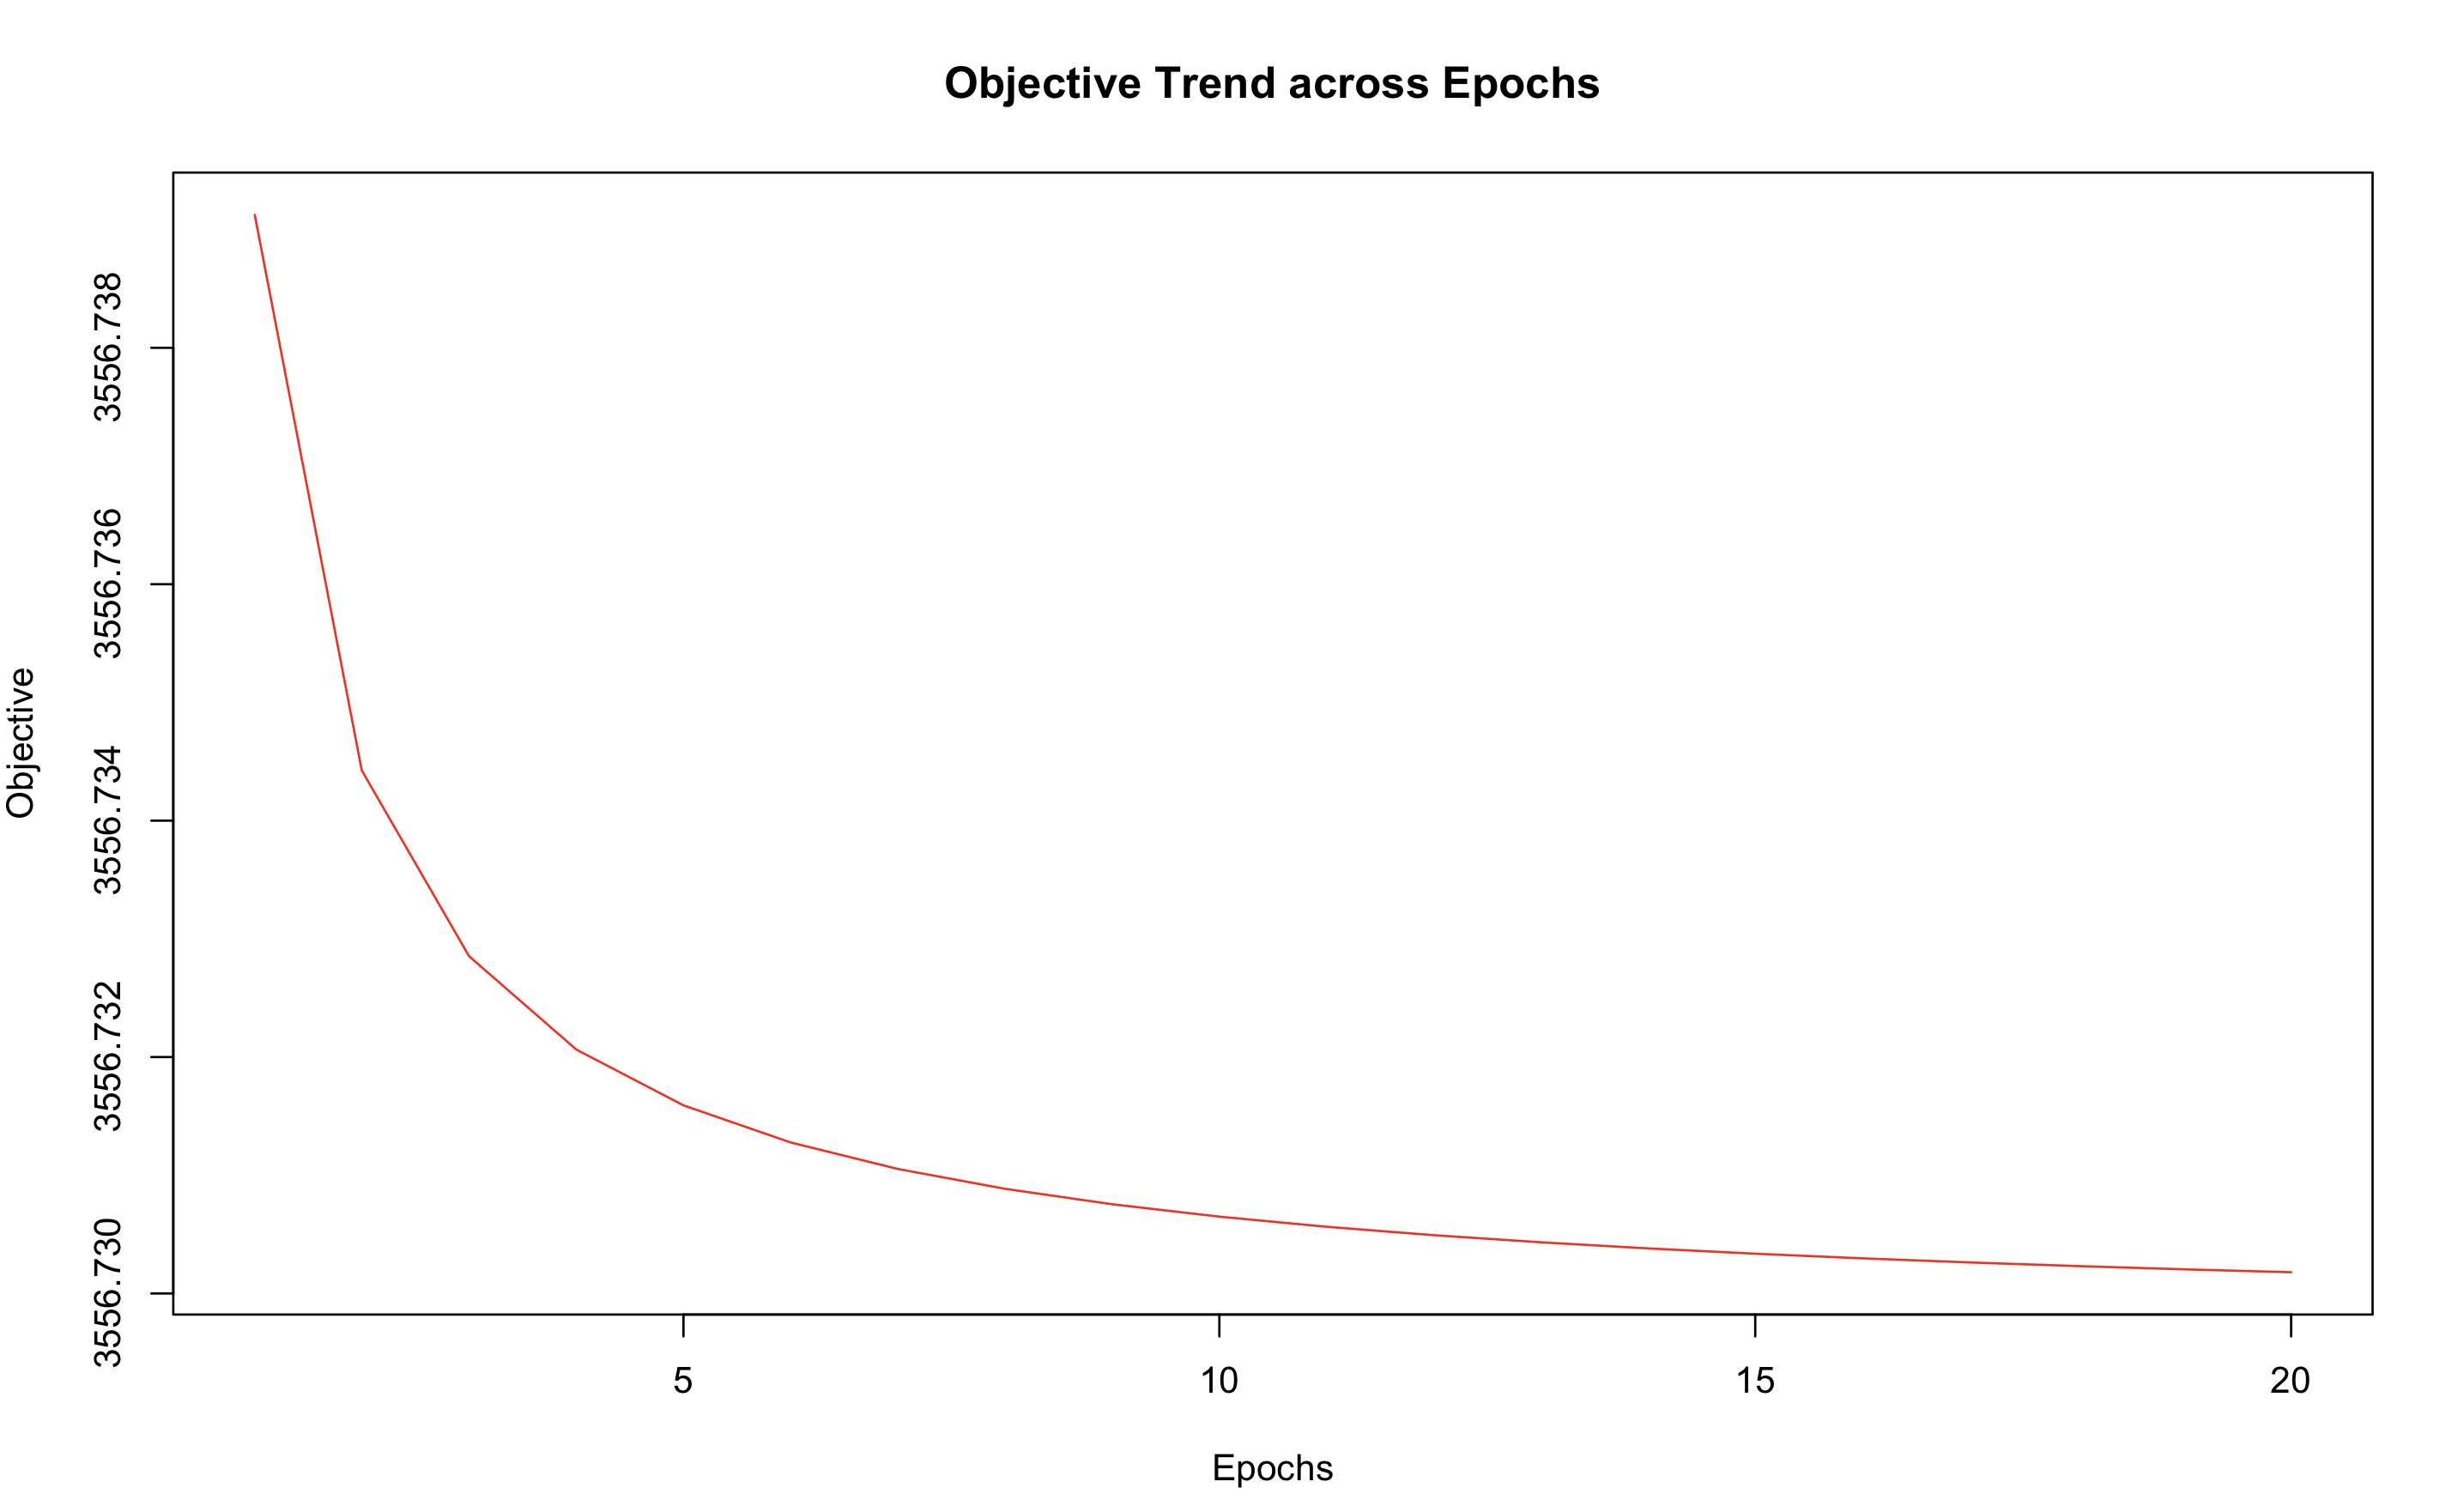
\includegraphics[width=5.5in]{ObjectiveTrend.png}
\caption{Plot of the objective}
\label{logl}
\end{figure}

\end{enumerate}




%%% Local Variables:
%%% mode: latex
%%% TeX-master: "hw6"
%%% End:
